\subsection{Desired properties}

We now define two desired properties of a non-interactive blockchain proof
protocol, \emph{succinctness} and \emph{security}.

\begin{definition}{(Security)}
A \emph{blockchain proof protocol} $(P, V)$ about a predicate $Q$ is
\emph{secure} if for all environments and for all PPT adversaries
$\mathcal{A}$ and for all rounds $r \geq \eta k$, if $V$ receives a proof at the
beginning of round $r$, then the output of $V$ at the end of round $r$ has the
following constraints:
\begin{itemize}
  \item If the output of $V$ is \emph{false}, then the evaluation of $Q(\chain)$
        for \emph{all} honest parties must be \emph{false} at the end of round
        $r - \eta k$.
  \item If the output of $V$ is \emph{true}, then the evaluation of $Q(\chain)$
        for \emph{all} honest parties must be \emph{true} at the end of round
        $r + \eta k$.
\end{itemize}
\end{definition}

\begin{figure}
    \caption{The truth value of a fixed predicate $Q$ about the blockchain, as
             seen from the point of view of $5$ honest nodes, drawn on the
             vertical axis, over time, drawn as the horizontal axis. The truth
             value evolves over time starting as \emph{false} at the beginning,
             indicated by a dashed red line. At some point in time $t_0$, the
             predicate is ready to be evaluated as \emph{true}, indicated by the
             solid blue line. The various honest nodes each realize this
             independently over a period of $\eta k$ duration, shaded in gray.
             The predicate remains \emph{false} for everyone before $t_0$ and
             \emph{true} for everyone after $t_0 + \eta k$.}
    \centering
    \iftwocolumn
        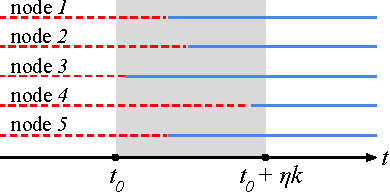
\includegraphics[width=\columnwidth,keepaspectratio]{figures/predicate-evolution.pdf}
    \else
        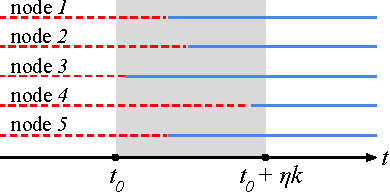
\includegraphics[width=0.4\columnwidth,keepaspectratio]{figures/predicate-evolution.pdf}
    \fi
    \label{fig.evolution}
\end{figure}

Some explanation is needed for the rationale of the above definition. The
parameter $\eta$ is borrowed from the Backbone~\cite{backbone} work and
indicates the rate at which new blocks are produced, i.e., the number of rounds
needed on average to produce a block. If the scheme is secure, this means that
the output of the verifier should match the output of a \emph{potential honest
full node}. However, in various executions, not all potential honest full node
behaviors will be instantiated. Therefore, we require that, if the output of the
proof verifier is \emph{true} then, consistently with honest behavior, all other
honest full nodes will converge to the value \emph{true}. Conversely, if the
output of the proof verifier is \emph{false} then, consistently with honest
behavior, all honest full nodes must not have indicated \emph{true} sufficiently
long in the past. The period $\eta k$ is the period needed for obtaining
sufficient confirmations ($k$) in a blockchain system. This is illustrated in
Figure~\ref{fig.evolution}. A predicate's value has the potential of being
\emph{true} as seen by an honest party starting at time $t_0$. Before time
$t_0$, all honest parties agree that the predicate is \emph{false}. It takes
$\eta k$ time for all parties to agree that the predicate is \emph{true}, which
is certain after time $t_0 + \eta k$. The adversary may be able to convince the
verifier that the predicate has any value during the period from $t_0$ to
$t_0 + \eta k$. However, our security definition mandates that before time $t_0$
the verifier will necessarily output \emph{false} and after time $t_0 + \eta k$
the verifier will necessarily output \emph{true}.

\begin{definition}{(Succinctness)}
A \emph{blockchain proof protocol} $(P, V)$ about a predicate $Q$ is
\emph{succinct} if for all PPT provers $\mathcal{A}$, any proof $\pi$ produced
by $\mathcal{A}$ at some round $r$, the verifier $V$ only reads a
$O(polylog(r))$-sized portion of $\pi$.
\end{definition}

It is easy to construct a \emph{secure but not succinct} protocol for any
computable predicate $Q$: The prover provides the entire chain $\chain$ as a
proof and the verifier simply selects the longest chain: by the
\emph{common-prefix property} of the backbone protocol (c.f.~\cite{backbone}),
this is consistent with the view of every honest party (as long as $Q$ depends
only on a \emph{prefix} of the chain, as we explain in more detail shortly). In
fact this is how widely-used cryptocurrency clients (including SPV clients)
operate today.

It is also easy to build \emph{succinct but insecure} clients: The prover simply
sends the predicate value directly. This is roughly what hosted wallets
do~\cite{sok}.

The challenge we will solve is to provide a non-interactive protocol that at the
same time achieves security and (optimistic) succinctness over a large class of
useful predicates.
